\documentclass[svgnames,table,,aspectratio=169]{beamer}
%\documentclass[svgnames,table,handout,aspectratio=129]{beamer}
\usepackage{hhline}
\usepackage{etoolbox}
\usepackage{tikz}
\usepackage{mathtools}
\usepackage{amssymb}
%\usepackage{/usr/lib64/R/share/texmf/Sweave}
\usepackage{polynom}
\usepackage{qrcode}


%\input{latexdefinitions}
\definecolor{georgiaRed}{RGB}{100,0,00}
\definecolor{mediumGray}{gray}{0.6}



\usetheme{Frankfurt}%
%\usetheme{Warsaw}%
%\useoutertheme{smoothbars}


%\usecolortheme{seagull}
\usecolortheme{beaver}
\logo{\includegraphics[height=.125in]{ugaLogo}}

% Note that the colour definitions are given in the latexDefinitions
% file.
\setbeamercolor{palette primary}{fg=georgiaRed,bg=white}
\setbeamercolor{palette secondary}{fg=georgiaRed,bg=white}
\setbeamercolor{palette tertiary}{fg=georgiaRed,bg=white}
\setbeamercolor{palette quaternary}{bg=mediumGray,fg=black}
\setbeamercolor{block title}{fg=white,bg=georgiaRed}
\setbeamercolor{block body}{fg=black,bg=black!10}
\setbeamercolor{titlelike}{bg=georgiaRed,fg=white} % parent=palette quaternary}

% Define the variable to determine whether or not the clicker quizzes
% are visible in the resulting output.
\newtoggle{clicker}
\toggletrue{clicker}
%\togglefalse{clicker}


% To display a lecture uncomment out the "includeonly" line below to
% match the name of the file. You do not have to do anything with the
% lecture line below and can leave it commented out. It is in place
% because at one time we had multiple lectures within a file, but that
% has been changed.



\mode<presentation>{
  \setbeamercovered{invisible}
  \setbeameroption{hide notes}
}

\mode<handout>{
 
  \usepackage{pgfpages}
  %\pgfpagesuselayout{4 on 1}[letterpaper, border shrink=5mm]
  \pgfpagesuselayout{resize to}[letterpaper,border shrink=5mm]
  \setbeameroption{show notes}


  %\pgfpagesphysicalpageoptions{logical pages=2,physical
  %height=\pgfpageoptionheight,physical width=\pgfpageoptionwidth}
  % Set up the pages for notes.
  % This idea and some code came from
  % http://www.guidodiepen.nl/2009/07/creating-latex-beamer-handouts-with-notes/



  \pgfpagesdeclarelayout{3 on 1 with notes} {
    \edef\pgfpageoptionheight{11in} %\the\paperheight}
    \edef\pgfpageoptionwidth{8.5in} %\the\paperwidth}
    \edef\pgfpageoptionborder{0pt}
  }

  {

	\AtBeginDocument{
      \newbox\notesbox
      \setbox\notesbox=\vbox{
        \hsize=\paperwidth
        \vskip-2.5cm\hskip-5cm\vbox{
          \textcolor{light-gray}{\hrule width 12.6cm\vskip0.5cm}
          \textcolor{light-gray}{\hrule width 12.6cm\vskip0.5cm}
          \textcolor{light-gray}{\hrule width 12.6cm\vskip0.5cm}
          \textcolor{light-gray}{\hrule width 12.6cm\vskip0.5cm}
          \textcolor{light-gray}{\hrule width 12.6cm\vskip0.5cm}
          \textcolor{light-gray}{\hrule width 12.6cm\vskip0.5cm}
          \textcolor{light-gray}{\hrule width 12.6cm\vskip0.5cm}
          \textcolor{light-gray}{\hrule width 12.6cm\vskip0.5cm}
          \textcolor{light-gray}{\hrule width 12.6cm\vskip0.5cm}
          \textcolor{light-gray}{\hrule width 12.6cm\vskip0.5cm}
          \textcolor{light-gray}{\hrule width 12.6cm\vskip0.5cm}
          \textcolor{light-gray}{\hrule width 12.6cm\vskip0.5cm}
          \textcolor{light-gray}{\hrule width 12.6cm\vskip0.5cm}
          \textcolor{light-gray}{\hrule width 12.6cm\vskip0.5cm}
          \textcolor{light-gray}{\hrule width 12.6cm\vskip0.5cm}
          \textcolor{light-gray}{\hrule width 12.6cm\vskip0.5cm}
          \textcolor{light-gray}{\hrule width 12.6cm\vskip0.5cm}
          \textcolor{light-gray}{\hrule width 12.6cm\vskip0.5cm}
          \textcolor{light-gray}{\hrule width 12.6cm\vskip0.5cm}

          \vspace*{-9.75cm}
          \textcolor{light-gray}{\rule[-1.0cm]{1pt}{9.25cm}\hskip0.5cm}
          \textcolor{light-gray}{\rule[-1.0cm]{1pt}{9.25cm}\hskip0.5cm}
          \textcolor{light-gray}{\rule[-1.0cm]{1pt}{9.25cm}\hskip0.5cm}
          \textcolor{light-gray}{\rule[-1.0cm]{1pt}{9.25cm}\hskip0.5cm}
          \textcolor{light-gray}{\rule[-1.0cm]{1pt}{9.25cm}\hskip0.5cm}
          \textcolor{light-gray}{\rule[-1.0cm]{1pt}{9.25cm}\hskip0.5cm}
          \textcolor{light-gray}{\rule[-1.0cm]{1pt}{9.25cm}\hskip0.5cm}
          \textcolor{light-gray}{\rule[-1.0cm]{1pt}{9.25cm}\hskip0.5cm}
          \textcolor{light-gray}{\rule[-1.0cm]{1pt}{9.25cm}\hskip0.5cm}
          \textcolor{light-gray}{\rule[-1.0cm]{1pt}{9.25cm}\hskip0.5cm}
          \textcolor{light-gray}{\rule[-1.0cm]{1pt}{9.25cm}\hskip0.5cm}
          \textcolor{light-gray}{\rule[-1.0cm]{1pt}{9.25cm}\hskip0.5cm}
          \textcolor{light-gray}{\rule[-1.0cm]{1pt}{9.25cm}\hskip0.5cm}
          \textcolor{light-gray}{\rule[-1.0cm]{1pt}{9.25cm}\hskip0.5cm}
          \textcolor{light-gray}{\rule[-1.0cm]{1pt}{9.25cm}\hskip0.5cm}
          \textcolor{light-gray}{\rule[-1.0cm]{1pt}{9.25cm}\hskip0.5cm}
          \textcolor{light-gray}{\rule[-1.0cm]{1pt}{9.25cm}\hskip0.5cm}
          \textcolor{light-gray}{\rule[-1.0cm]{1pt}{9.25cm}\hskip0.5cm}
          \textcolor{light-gray}{\rule[-1.0cm]{1pt}{9.25cm}\hskip0.5cm}
          \textcolor{light-gray}{\rule[-1.0cm]{1pt}{9.25cm}\hskip0.5cm}

        }

      }

    \pgfpagesphysicalpageoptions
    {%
      logical pages=6,%
      physical height=\pgfpageoptionheight,%
      physical width=\pgfpageoptionwidth,%
      last logical shipout=3%
    }
    
    \pgfpageslogicalpageoptions{1}
    {%
      border shrink=\pgfpageoptionborder,%
      resized width=.5\pgfphysicalwidth,%
      resized height=.33\pgfphysicalheight,%
      center=\pgfpoint{.25\pgfphysicalwidth}{.82\pgfphysicalheight}%
    }%
    \pgfpageslogicalpageoptions{2}
    {%
      border shrink=\pgfpageoptionborder,%
      resized width=.5\pgfphysicalwidth,%
      resized height=.33\pgfphysicalheight,%
      center=\pgfpoint{.25\pgfphysicalwidth}{.47\pgfphysicalheight}%
    }%
    \pgfpageslogicalpageoptions{3}
    {%
      border shrink=\pgfpageoptionborder,%
      resized width=.5\pgfphysicalwidth,%
      resized height=.33\pgfphysicalheight,%
      center=\pgfpoint{.25\pgfphysicalwidth}{.17\pgfphysicalheight}%
    }%	
	\pgfpageslogicalpageoptions{4}
    {%
      border shrink=\pgfpageoptionborder,%
      resized width=.5\pgfphysicalwidth,%
      resized height=.33\pgfphysicalheight,%
      center=\pgfpoint{.85\pgfphysicalwidth}{.82\pgfphysicalheight},%
      copy from=4
    }%
    \pgfpageslogicalpageoptions{5}
    {%
      border shrink=\pgfpageoptionborder,%
      resized width=.5\pgfphysicalwidth,%
      resized height=.33\pgfphysicalheight,%
      center=\pgfpoint{.85\pgfphysicalwidth}{.47\pgfphysicalheight},%
      copy from=5
    }%
    \pgfpageslogicalpageoptions{6}
    {%
      border shrink=\pgfpageoptionborder,%
      resized width=.5\pgfphysicalwidth,%
      resized height=.33\pgfphysicalheight,%
      center=\pgfpoint{.85\pgfphysicalwidth}{.17\pgfphysicalheight},%
      copy from=6
    }%
    
      \pgfpagesshipoutlogicalpage{4}\copy\notesbox
      \pgfpagesshipoutlogicalpage{5}\copy\notesbox
      \pgfpagesshipoutlogicalpage{6}\copy\notesbox
    }
  }

  \pgfpagesuselayout{3 on 1 with notes}

}

\setbeamercolor{upper separation line head}{bg=red}
\setbeamercolor{headline}{bg=red}
\setbeamertemplate{headline}
{%
\begin{beamercolorbox}{section in head/foot}
\insertsectionnavigationhorizontal{.75\textwidth}{}{}
\hfill \insertpagenumber /\insertdocumentendpage
\end{beamercolorbox}%
}
\setbeamercolor{section number projected}{bg=red,fg=black}
\setbeamercolor{subsection number projected}{bg=red,fg=black}
%\setbeamercolor{frametitle}{bg=lightgray,fg=black}

\setbeamertemplate{itemize item}{\color{georgiaRed}$\blacklozenge$}
\setbeamertemplate{itemize subitem}{\color{georgiaRed}$\blacktriangleright$}

\newcommand{\dotfield}[2]{%
  \begin{tikzpicture}[y=0.25cm, x=0.25cm,font=\sffamily]
    \foreach \y in {0,...,#2} {
      \foreach \x in {0,...,#1} {
        \draw[fill=georgiaRed,opacity=0.1] (\x,\y)  circle [radius=0.03em];
      }
    }
  \end{tikzpicture}
}

\newcommand{\twoByTwo}[4]{%
  \left[
    \begin{array}{rr}
      #1 & #2 \\
      #3 & #4 \\
    \end{array}
  \right]
}

\newcommand{\threeByThree}[9]{%
  \left[
    \begin{array}{rrr}
      #1 & #2 & #3 \\
      #4 & #5 & #6 \\
      #7 & #8 & #9
    \end{array}
  \right]
}

\newcommand{\columnVector}[1]{%
  \left[
    \begin{array}{r}
    #1                           
    \end{array}
  \right]
}


\begin{document}



\author{\textsc{T. Alli$^{a}$, K. Black$^{a}$}}
\institute{$^a$Department of Mathematics, University of Georgia, GA}
\subject{Linear Algebra}
\keywords{Linear Transformation, Vectors, Matrices, Linear Algebra}

%\lecture{Partial Fractions}{partial-fractions}
%\section{Rational Functions}

\title{Section 4.1: The Determinant}
\subtitle{Another Tool To Determine If A Matrix Is Invertible}


\date{} % {\today}

\begin{frame}
  \titlepage
\end{frame}

\begin{frame}{Outline}
  \tableofcontents
\end{frame}


\section{Goals}

\begin{frame}{Goals}

  \begin{itemize}
  \item Calculate the determinant of a square matrix.
  \item Use the determinant to determine if a matrix is invertible.
  \item Determine the determinant of the product of matrices.
  \item Determine the determinant of a matrices for special cases.
  \item Calculate the transpose of a matrix.
  \end{itemize}

\end{frame}

\section{Determinant Of A Two-By-Two Matrix}

\begin{frame}{System Of Two Equations}

  \begin{eqnarray*}
    3x + 2y & = & 7 \\
    8x + 4y & = & 10.
  \end{eqnarray*}

  \uncover<2->{
    
    \begin{eqnarray*}
      (4) \left( 3x + 2y \right)  & = & (4) \left( 7 \right) \\
      (2) \left( 8x + 4y  \right) & = & (2) \left( 10 \right).
    \end{eqnarray*}
    
  }

  \uncover<3->{
    
    \begin{eqnarray*}
      (4) \left( 3x + 2y \right)  - (2) \left( 8x + 4y  \right)
      & = & (4) \left( 7 \right) - (2) \left( 10 \right).
    \end{eqnarray*}
    
  }

  \dotfield{60}{10}
  
\end{frame}

\begin{frame}{System Of Two Equations}

  \begin{eqnarray*}
    ax + by & = & \#_1 \\
    cx + dy & = & \#_2.
  \end{eqnarray*}

  \uncover<2->{
    
    \begin{eqnarray*}
      (d) \left( ax + by \right)  & = & (d) \left( \#_1 \right) \\
      (b) \left( cx + dy  \right) & = & (b) \left( \#_2 \right).
    \end{eqnarray*}
    
  }

  \uncover<2->{
    
    \begin{eqnarray*}
      (d) \left( ax + by \right) - (b) \left( cx + dy  \right)
      & = & (d) \left( \#_1 \right)  - (b) \left( \#_2 \right).
    \end{eqnarray*}
    
  }

  \dotfield{60}{14}

\end{frame}

\begin{frame}{Geometric View}

  Suppose we have two vectors,
  \begin{eqnarray*}
    \vec{u} = \columnVector{a \\ c }, & & \vec{v} = \columnVector{b \\ d}.
  \end{eqnarray*}

  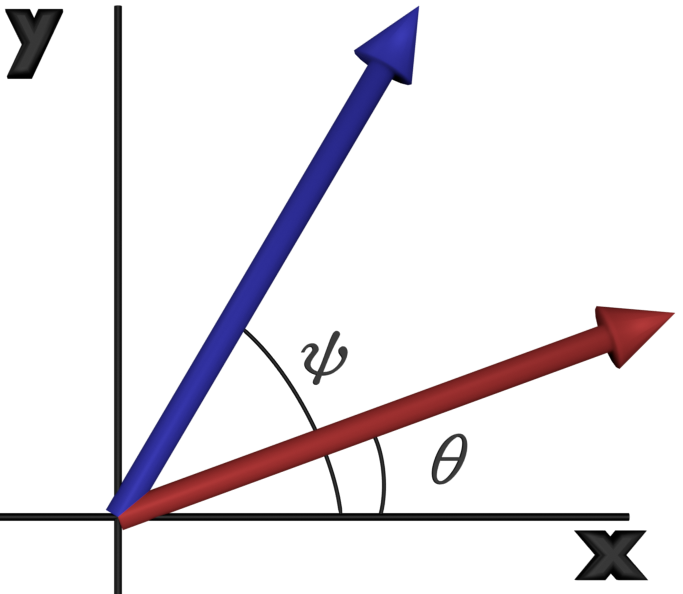
\includegraphics[height=5cm]{areaTwoVectors}

  \vfill
  
\end{frame}

\begin{frame}{Geometric View}

  Suppose we have two vectors,
  \begin{eqnarray*}
    \vec{u} = \columnVector{a \\ c }, & & \vec{v} = \columnVector{b \\ d}.
  \end{eqnarray*}

  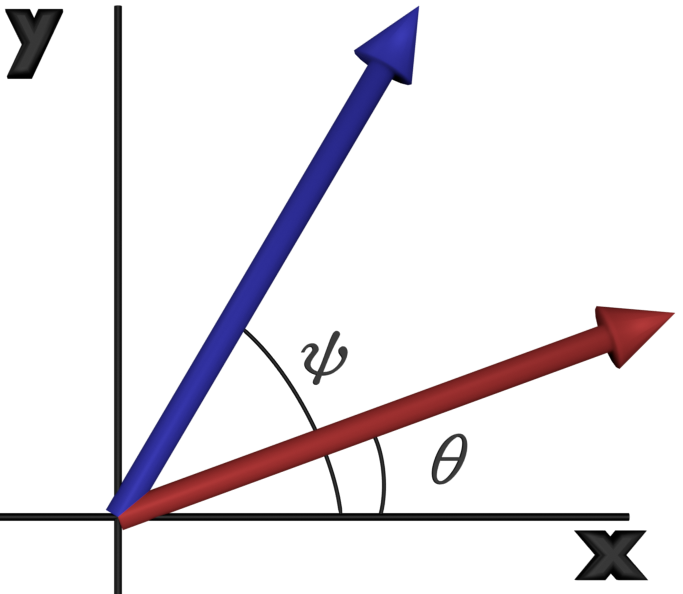
\includegraphics[height=5cm]{areaTwoVectors}

  \vfill
  
\end{frame}

\begin{frame}{Example: Is There A Unique Solution?}

  \begin{eqnarray*}
     2x + 2y & = & 7, \\
    -x  + 4y & = & 2.
  \end{eqnarray*}

  \dotfield{60}{22}
  
\end{frame}

\begin{frame}{Example: Is There A Unique Solution?}

  \begin{eqnarray*}
     3x + 2y & = & 7, \\
    -6x - 4y & = & 2.
  \end{eqnarray*}

  \dotfield{60}{22}
  
\end{frame}

\section{Summary Of Properties of Determinants}

\begin{frame}{Properties Of Determinants}

  \begin{enumerate}
  \item Only exist for square matrices.
  \item Adding a multiple of a row to a different row does not change
    the determinant.
  \item Multiplying a row by a number, $c$, multiplies the determinant
    by $c$.
  \item Swapping two rows multiplies the determinant by -1.
  \item The determinant of the identity matrix is 1.
  \end{enumerate}
  
\end{frame}

\begin{frame}{Example: Row Operations To Calculate The Determinant}

  \begin{eqnarray*}
     2x + 2y & = & 7, \\
    -x  + 4y & = & 2.
  \end{eqnarray*}

  \dotfield{60}{22}
  
\end{frame}

\begin{frame}{Example: Row Operations To Calculate The Determinant}

  \begin{eqnarray*}
     3x + z & = & 8, \\
    -6x + y + 3z & = & 4, \\
    12x + 2y + 2z & = & -1
  \end{eqnarray*}

  \dotfield{60}{22}

  % -36
  
\end{frame}


\section{Special Cases}

\begin{frame}{Upper-Triangular, Lower-Triangular, Diagonal Matrices}

  \begin{columns}
    \column{0.33\textwidth}

    Upper-Triangular Matrix
    \begin{eqnarray*}
      \left[
      \begin{array}{rrrrr}
        * & * & * & * & * \\
        0 & * & * & * & * \\
        0 & 0 & * & * & * \\
        0 & 0 & 0 & * & * \\
        0 & 0 & 0 & 0 & * 
      \end{array}
      \right]
    \end{eqnarray*}

    \column{0.33\textwidth}

    Diagonal Matrix
    \begin{eqnarray*}
      \left[
      \begin{array}{rrrrr}
        * & 0 & 0 & 0 & 0 \\
        0 & * & 0 & 0 & 0 \\
        0 & 0 & * & 0 & 0 \\
        0 & 0 & 0 & * & 0 \\
        0 & 0 & 0 & 0 & * 
      \end{array}
      \right]
    \end{eqnarray*}

    \column{0.33\textwidth}

    Lower-Triangular Matrix
    \begin{eqnarray*}
      \left[
      \begin{array}{rrrrr}
        * & 0 & 0 & 0 & 0 \\
        * & * & 0 & 0 & 0 \\
        * & * & * & 0 & 0 \\
        * & * & * & * & 0 \\
        * & * & * & * & * 
      \end{array}
      \right]
    \end{eqnarray*}

    
  \end{columns}
  
\end{frame}

\begin{frame}{Determinants Of Upper-Triangular, Lower-Triangular, and
    Diagonal Matrices}

  \begin{eqnarray*}
    \left[
    \begin{array}{rrrrr}
      * & * & * & * & * \\
      0 & * & * & * & * \\
      0 & 0 & * & * & * \\
      0 & 0 & 0 & * & * \\
      0 & 0 & 0 & 0 & * 
    \end{array}
    \right]
  \end{eqnarray*}

  \dotfield{60}{20}

\end{frame}

\section{Properties Of The Determinant}

\begin{frame}{If The Determinant Is Zero}

  If the determinant of a matrix is zero, then it is not
  invertible. Otherwise it is invertible.

  \dotfield{60}{20}
  
\end{frame}

\begin{frame}{Determinant Of The Product Of Two Matrices}

  If $A$ and $B$ are square matrices then
  $\det(AB)=\det(A)\det(B)$. (See p. 196)
  
  \dotfield{60}{20}
  
\end{frame}

\begin{frame}{Determinant Of A Matrix Raised To A Power}

  If $A$ is a square matrix then
  $\det(A^n)= \left(\det(A)\right)^n$.
  
  \dotfield{60}{20}
  
  
\end{frame}

\begin{frame}{Determinant Of The Inverse Of A Matrix}

  If $A$ is an invertible, square matrix then
  $\det(A^{-1})= \frac{1}{\det(A)}$.
  
  \dotfield{60}{20}
  
  
\end{frame}
  

\section{The Transpose}

\begin{frame}{The Transpose}

  The transpose of a matrix is found by swapping the rows of a matrix
  and making them the columns of the new matrix.

  \begin{eqnarray*}
    \left[
    \begin{array}{rrrrr}
      3 & 8 &  7 & -1 & 2 \\
      1 & 5 & -1 &  4 & 9 \\
      6 & 2 & 10 &  3 & 22
    \end{array}
    \right]^T
  \end{eqnarray*}

  \dotfield{60}{18}
  
\end{frame}

\begin{frame}{Transpose Of The Product Of Two Matrices}

  \begin{eqnarray*}
    (AB)^T & = & B^T A^T.
  \end{eqnarray*}
  (see p. 200)

  \dotfield{60}{22}
  
\end{frame}

\begin{frame}{Determinant Of The Transpose Of A Matrix}

  \begin{eqnarray*}
    \det\left(A^T\right) & = & \det(A).
  \end{eqnarray*}
  (see p. 200)

  \dotfield{60}{22}
  
\end{frame}


\begin{frame}{Blank Page}
  \dotfield{60}{24}
\end{frame}


\end{document}
